\documentclass[final,t]{beamer}
\mode<presentation>
{
%  \usetheme{Warsaw}
%  \usetheme{Aachen}
%  \usetheme{Oldi6}
%  \usetheme{I6td}
  \usetheme{I6dv}
%  \usetheme{I6pd}
%  \usetheme{I6pd2}
}
% additional settings
\setbeamerfont{itemize}{size=\normalsize}
\setbeamerfont{itemize/enumerate body}{size=\normalsize}
\setbeamerfont{itemize/enumerate subbody}{size=\normalsize}

% additional packages
\usepackage{times}
\usepackage{amsmath,amsthm, amssymb, latexsym}
\usepackage{exscale}
%\boldmath
\usepackage{booktabs, array}
%\usepackage{rotating} %sideways environment
\usepackage[english]{babel}
\usepackage[latin1]{inputenc}
%\usepackage[orientation=landscape,size=custom,width=200,height=120,scale=1.9]{beamerposter}
\usepackage[orientation=landscape,size=custom,width=121.9,height=121.9,scale=1.9]{beamerposter}
%\usepackage[orientation=landscape,size=a0,scale=1.9]{beamerposter}


\listfiles
\graphicspath{{figures/}}
% Display a grid to help align images
%\beamertemplategridbackground[1cm]

\usepackage{todonotes}

\title{\huge An atlas for the genomes of\\ \emph{Phytophthora infestans}}
%\author[Knaus et al.]{Brian J. Knaus$^{1}$, Javier F. Tabima$^{2}$, Howard S. Judelson and Niklaus J. Gr\"{u}nwald$^{1, 2}$}
\author[Knaus et al.]{Brian J. Knaus$^{1}$, Javier F. Tabima$^{2}$ and Niklaus J. Gr\"{u}nwald$^{1, 2}$}
\institute[USDA-ARS, OSU, UCR]{$^{1}$Horticultural Crops Research Unit, USDA Agricultural Research Service\\ $^{2}$Department of Botany and Plant Pathology, Oregon State University}
\date[August 9, 2014]{August 9, 2014}

% abbreviations
\usepackage{xspace}
\makeatletter
\DeclareRobustCommand\onedot{\futurelet\@let@token\@onedot}
\def\@onedot{\ifx\@let@token.\else.\null\fi\xspace}
\def\eg{{e.g}\onedot} \def\Eg{{E.g}\onedot}
\def\ie{{i.e}\onedot} \def\Ie{{I.e}\onedot}
\def\cf{{c.f}\onedot} \def\Cf{{C.f}\onedot}
\def\etc{{etc}\onedot}
\def\vs{{vs}\onedot}
\def\wrt{w.r.t\onedot}
\def\dof{d.o.f\onedot}
\def\etal{{et al}\onedot}
\makeatother

%%%%%%%%%%%%%%%%%%%%%%%%%%%%%%%%%%%%%%%%%%%%%%%%%%%%%%%%%%%%%%%%%%%%%%%%%%%%%%%%%%%%%%%%%%%%%%%%%%%%%%%%%%%%
%%%%%%%%%%%%%%%%%%%%%%%%%%%%%%%%%%%%%%%%%%%%%%%%%%%%%%%%%%%%%%%%%%%%%%%%%%%%%%%%%%%%%%%%%%%%%%%%%%%%%%%%%%%%
\begin{document}
\begin{frame}{} 
  \begin{columns}[t]
    \begin{column}{.28\linewidth}

      %%%%%%%%%%%%%%%%%%%%%%%%%%%%%%%%%%%%%%%%%%%%%%%%%%%%%%%%%%%%%%%%%%%%%%%%%%%%%%%%%%%%%%%%%%%%%%%%%%%%%%%%%%%%

%      \begin{block}{Introduction}
      \begin{block}{Abstract}
The causative agent of the Irish Potato Famine, \emph{Phytophthora infestans}, continues to cost billions of dollars in mitigation and crop loss, annually.  Late blight of potato and tomato, therefore, plays an important role in world food security.  To date, 26 genomes of this pathogen have been sequenced.  Lineages US-8 and US-22 have been characterized as having resistance to the commonly used fungicide metalaxyl.  The mode of action for metalaxyl has been reported to include transcription, such that RNA polymerases, and their associated proteins, have been promoted as candidate loci.  We present a genome-wide survey of markers which bioinformatically differentiate these fungicide resistant lineages from susceptible lineages and characterize whether these candidate loci contain polymorphisms which segregate in a manner which may confer resistance.
      \end{block}

%Populations occur as assumedly clonal lineages which had been anciently sexually recombinant.

      %%%%%%%%%%%%%%%%%%%%%%%%%%%%%%%%%%%%%%%%%%%%%%%%%%%%%%%%%%%%%%%%%%%%%%%%%%%%%%%%%%%%%%%%%%%%%%%%%%%%%%%%%%%%
      
  \begin{block}{Bioinformatic methods}
    \begin{itemize}
      \item Sequence reads (Illumina of various lengths and Roche 454) were acquired through publicly available archives as well as novel sequencing
      \item Reads were mapped to the T30-4 reference with bowtie2
      \item Variants were called using SAMtools
      \item Variants were post-processed for quality and coverage with custom code
    \end{itemize}
  \end{block}

      %%%%%%%%%%%%%%%%%%%%%%%%%%%%%%%%%%%%%%%%%%%%%%%%%%%%%%%%%%%%%%%%%%%%%%%%%%%%%%%%%%%%%%%%%%%%%%%%%%%%%%%%%%%%
      \begin{block}{Genome summaries}
\missingfigure{Barplot of RR, RA, AA.}

      \end{block}

    \end{column}
      %%%%%%%%%%%%%%%%%%%%%%%%%%%%%%%%%%%%%%%%%%%%%%%%%%%%%%%%%%%%%%%%%%%%%%%%%%%%%%%%%%%%%%%%%%%%%%%%%%%%%%%%%%%%

    \begin{column}{.4\linewidth}


      \begin{block}{Visualization of Supercontig 60}
        \begin{columns}[t]
          \begin{column}[T]{0.6\linewidth}
            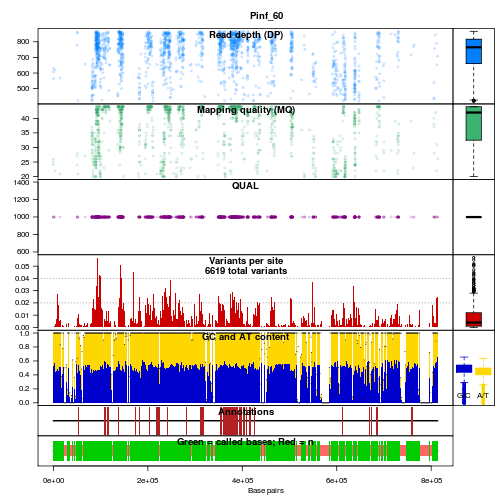
\includegraphics[width=0.9\linewidth, height=0.7\linewidth]{cplots3.png}
          \end{column}
          \begin{column}[T]{0.4\linewidth}
            Describe the plot.
            \begin{itemize}
              \item Filtered on read depth
              \item Filtered on quality (QUAL)
            \end{itemize}
          \end{column}
        \end{columns}
      \end{block}

      %%%%%%%%%%%%%%%%%%%%%%%%%%%%%%%%%%%%%%%%%%%%%%%%%%%%%%%%%%%%%%%%%%%%%%%%%%%%%%%%%%%%%%%%%%%%%%%%%%%%%%%%%%%%

      \begin{block}{Mitochondrial phylogeny of \emph{Phytophthora infestans}}
            Neighbor-joing tree based on Euclidian distances to describe relationships within \emph{Phytophthora infestans}.

        \begin{columns}[t]
          \begin{column}[T]{0.6\linewidth}
            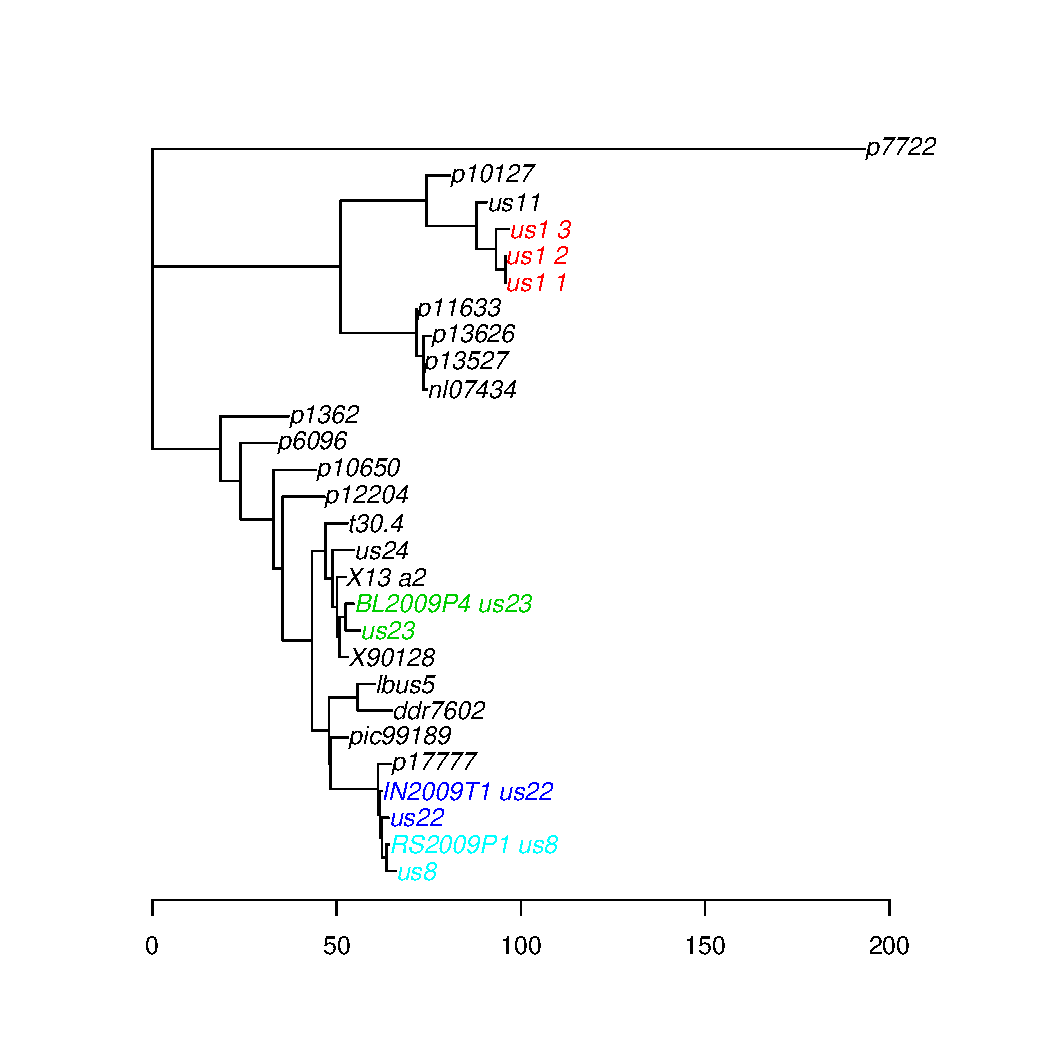
\includegraphics[width=0.9\linewidth, height=1.2\linewidth]{chromR7.pdf}
          \end{column}
          \begin{column}[T]{0.4\linewidth}
            \begin{itemize}
              \item \emph{P. mirabilis} (p7722) is the outgroup
              \item The \emph{Phytophthora} mitochondrion consists of 40,NNN nucleotides
              \item Lineage US-1 forms an independant clade (samples us1 1, us1 2 and us1 3 are the same lineage)
              \item Lineages US-8, US-22 and sample p17777 form a clade (assumedly all fungicide resistant)
%              \item other stuff
            \end{itemize}
          \end{column}
        \end{columns}
      \end{block}

      %%%%%%%%%%%%%%%%%%%%%%%%%%%%%%%%%%%%%%%%%%%%%%%%%%%%%%%%%%%%%%%%%%%%%%%%%%%%%%%%%%%%%%%%%%%%%%%%%%%%%%%%%%%%

      \begin{block}{Genotypic quality for Supercontig 60}
        \begin{columns}[t]
          \begin{column}[T]{0.6\linewidth}
            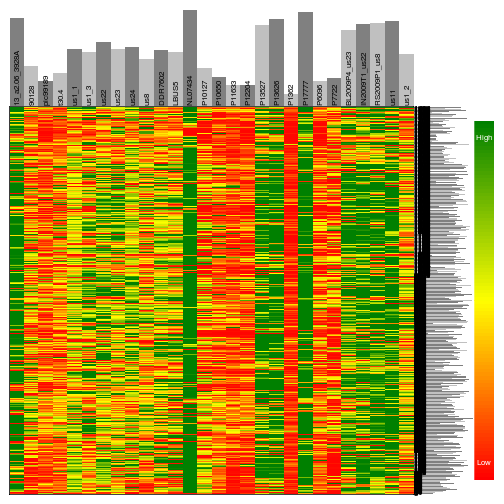
\includegraphics[width=0.9\linewidth, height=0.6\linewidth]{heatmap3.png}
          \end{column}
          \begin{column}[T]{0.4\linewidth}
            Summary of genotype qualities
            \begin{itemize}
%              \item Green represents a quality of 100, red represents a quality of 0
              \item Most genotypes are of intermediate quality
              \item Only genotypes of $\geq$100X coverage are of high quality (green)
              \item Most genotypes are of moderate quality
            \end{itemize}
          \end{column}
        \end{columns}
      \end{block}



      %%%%%%%%%%%%%%%%%%%%%%%%%%%%%%%%%%%%%%%%%%%%%%%%%%%%%%%

    \end{column}

    %%%%%%%%%%%%%%%%%%%%%%%%%%%%%%%
    
    \begin{column}{.28\linewidth}

  \begin{block}{Variants identifying fungicide resistant lineages (US-8 \& US-22)}
    \begin{table}
    \begin{tabular}{lc}
      \hline
        \textbf{Supercontig} & \textbf{Position} \\
      \hline
        Supercontig\_1.NN & nnn \\
        Supercontig\_1.NN & nnn \\
      \hline
    \end{tabular}
    \end{table}

  \end{block}
      
  \begin{block}{Discussion}
    Blah, blah and blah.

  \end{block}

%%%%%%%%%%%%%%%%%%%%%%%%%%%%%%%%%%%%%%%%%%%%%%%%%%%%%%%
                
      \begin{block}{Conclusions}
        \begin{itemize}
        \item Lineages characterized as having fungicide resistance (US-8 and US-22) form a clade
        \item \#N variants uniquely define this fungicide resistant clade (homozygote for versus homozygote against)
        \item Functional genomics will attempt to validate these candidates for fungicide resistance
%        \item Conclusion 3
        \end{itemize}
        \vspace{-1ex}
      \end{block}
%%%%%%%%%%%%%%%%%%%%%%%%%%%%%%%%%%%%%%%%%%%%%%%%%%%%%%%

      \begin{block}{Acknowledgements}
Funding was provided by USDA NIFA.
      \end{block}
%%%%%%%%%%%%%%%%%%%%%%%%%%%%%%%%%%%%%%%%%%%%%%%%%%%%%%%

    \end{column}
  \end{columns}
\end{frame}

\end{document}


%%%%%%%%%%%%%%%%%%%%%%%%%%%%%%%%%%%%%%%%%%%%%%%%%%%%%%%%%%%%%%%%%%%%%%%%%%%%%%%%%%%%%%%%%%%%%%%%%%%%
%%% Local Variables: 
%%% mode: latex
%%% TeX-PDF-mode: t
%%% End: 
